\documentclass[10pt,twocolumn,letterpaper]{article}

\usepackage{cvpr}
\usepackage{times}
\usepackage{epsfig}
\usepackage{graphicx}
\usepackage{amsmath}
\usepackage{amssymb}
\usepackage[utf8]{inputenc}
\usepackage[T1]{fontenc}


% Include other packages here, before hyperref.

% If you comment hyperref and then uncomment it, you should delete
% egpaper.aux before re-running latex.  (Or just hit 'q' on the first latex
% run, let it finish, and you should be clear).
\usepackage[breaklinks=true,bookmarks=false]{hyperref}

\cvprfinalcopy % *** Uncomment this line for the final submission

\def\cvprPaperID{****} % *** Enter the CVPR Paper ID here
\def\httilde{\mbox{\tt\raisebox{-.5ex}{\symbol{126}}}}

% Pages are numbered in submission mode, and unnumbered in camera-ready
%\ifcvprfinal\pagestyle{empty}\fi
\setcounter{page}{1}
\begin{document}

%%%%%%%%% TITLE
\title{Desenvolvimento de Aplicações em Assembly MIPS \\
	Universidade de Brasília\\
  \large Organização e Arquitetura de Computadores\\
  Turma B}
\author{Danielle Almeida Lima\\
14/0135740\\
Universidade de Brasília\\
{\tt\small almeidadani67@gmail.com}
% For a paper whose authors are all at the same institution,
% omit the following lines up until the closing ``}''.
% Additional authors and addresses can be added with ``\and'',
% just like the second author.
% To save space, use either the email address or home page, not both
\and
Samuel Venzi Lima Monteiro de Oliveira\\
14/0162241\\
Universidade de Brasília\\
{\tt\small samuel.venzi@me.com}
}

\maketitle
%\thispagestyle{empty}

%%%%%%%%% ABSTRACT
\begin{abstract}
   Estudo da linguagem Assembly por intermédio do desenvolvimento de uma
   agenda telefônica, a partir de metodologias otimizadas e efetivas.
   Análise de como uma linguagem de baixo nível pode afetar o desempenho
   e as vantagens e desvantagens causadas por esse tipo de linguagem no
   sistema operacional. A elaboração deste trabalho propiciou uma maior
   abstração na relação entre linguagem e desempenho no sistema
   operacional, bem como qual metodologia de organização e arquitetura
   de computadores é mais eficiente dado um problema específico.
\end{abstract}

%%%%%%%%% BODY TEXT
\section{Introdução}

A linguagem de máquina é dada por um conjunto de instruções, tal
que cada instrução é uma palavra da máquina. A Unidade Central de Processamento
(CPU) é projetada com o intuito de reconhecer instruções codificadas como padrão
de bits. O código de máquina é o ponto inicial para projeto de uma arquitetura, 
a qual é essencial na definição da qualidade do sistema como um todo. 

%-------------------------------------------------------------------------
\subsection{Arquitetura de Computadores}

Há duas abordagens para o conjunto de instruções, a RISC (Reduced Instruction
Set Computer) e a CISC (Complex Instruction Set Computer). A arquitetura RISC
visa um conjunto simples de instruções para resultar em uma CPU simples, barata
e rápida, que acessa mais os registradores, já a arquitetura CISC está relacionada a instruções complexas que demandam uma grande quantidade de ciclos para serem executadas.
As operações realizadas com registradores são mais rápidas do que as com a memória.

A arquitetura do conjunto de instruções trabalhada é a MIPS (Microprocessor without Interlocked Pipeline Stages) baseada na arquitetura RISC, ou seja, do tipo load/store e usa poucos ciclos do processador para executar instruções. O padrão adotado da arquitetura é de 32 bits. Ademais, possui algumas características que simplificam a sua implementação, como todas as operações da Unidade Lógica e Aritmética (ULA) são realizadas apenas pelos registradores, logo a memória só é acessada através das instruções load e store e as instruções possuem poucos formatos e todas são do mesmo tamanho.

\begin{table}[h]
\renewcommand{\tablename}{Tabela}
\begin{center}
\begin{tabular}{|l|c||c|}
\hline
Nome & Número & Uso \\
\hline\hline
\$zero & 0 & valor zero (hardwire)\\
\$at & 1 & reservado para o montador\\
\$vo-\$v1 & 2-3 & retorno de valores de funções\\
\$ao-\$a3 & 4-7 & passagem de argumentos\\
\$to-\$t7 & 8-15 & dados temporários\\
\$so-\$s7 & 16-23 & dados temporários salvos\\
\$t8 & 24 & dados temporários\\
\$t9 & 25 & dados temporários\\
\$k0 & 26 & reservados para o sistema operacional\\
\$k1 & 27 & reservados para o sistema operacional\\
\$gp & 28 & ponteiro global\\
\$sp & 29 & ponteiro da pilha\\
\$fp & 30 & ponteiro de frame\\
\$ra & 31 & endereço de retorno\\
\hline
\end{tabular}
\end{center}
\caption{Organização dos registradores MIPS.}
\end{table}

A memória está organizada como um grande array unidimensional com endereços sequênciais, desse modo o índice do array é um endereço de memória. Apesar do endereçamento ser feito em byte (4 bits) o MIPS escreve em words (32 bits), assim todos os registradores possuem 32 bits de dados.

É utilizado o simulador MARS que é um ambiente de desenvolvimento integrado (IDE) que funciona como um montador com recursos de checagem semântica para produzir um programa em linguagem assembly. Um programa está estruturado basicamente neste simulador em duas áreas: .data para declaração de variáveis estáticas e .text que é a área das instruções.

Um projeto tem como objetivo maximizar o tempo, diminuir o custo e e minimizar o tempo de projeto, tendo como princípio que a simplicidade favorece a regularidade, quanto menor, mais rápido o programa, é necessário agilizar o caso comum e por fim um bom projeto exige bons compromissos.


\subsection{Tipos de Instruções}

Na arquitetura MIPS todas as instruções possuem o mesmo tamanho, o que as diferencia é o seu formato. As instruções são divididaas em três formatos: Tipo-R, Tipo-I e Tipo-J. A do Tipo-R está relacionada as operações da ULA, já as do Tipo-I estão relacionadas à transferência de dados e as do Tipo-J são usadas para desvios e saltos. As tabelas 2, 3, 4, 5 e 6 mostram as principais instruções, relacionadas com seus mnemônicos e seu significado.

\begin{table}[h]
\renewcommand{\tablename}{Tabela}
\begin{center}
\begin{tabular}{|l|c||c|}
\hline
Instrução & Exemplo & Significado \\
\hline\hline
add & add \$s1, \$s2, \$s3 & \$s1=\$s2+\$s3\\
subtract & sub \$s1, \$s2, \$s3 & \$s1=\$s2-\$s3\\
add immediate & addi \$s1, \$s2, 1 & \$s1=\$s2+1\\
\hline
\end{tabular}
\end{center}
\caption{Instruções para operações aritméticas.}
\end{table}

\begin{table}[h]
\renewcommand{\tablename}{Tabela}
\begin{center}
\begin{tabular}{|l|c||c|}
\hline
Instrução & Exemplo & Significado \\
\hline\hline
load word & lw \$s1, 0(\$s2) & \$s1=Memory[\$s2+0]\\
store word & sw \$s1, 0(\$s2) & Memory[\$s2+0]=\$s1\\
load byte & lb \$s1, 0(\$s2) & \$s1=Memory[\$s2+0]\\
store byte & sb \$s1, 0(\$s2) & Memory[\$s2+0]=\$s1\\
\hline
\end{tabular}
\end{center}
\caption{Instruções para transferência de dados.}
\end{table}

\begin{table}[h]
\renewcommand{\tablename}{Tabela}
\begin{center}
\begin{tabular}{|l|c||c|}
\hline
Instrução & Exemplo & Significado \\
\hline\hline
and & and \$s1, \$s2, \$s3 & \$s1=\$s2\&\$s3\\
or & and \$s1, \$s2, \$s3 & \$s1=\$s2 | \$s3\\
nor & nor \$s1, \$s2, \$s3 & \$s1=~(\$s2 | \$s3)\\
shift left logical & sll \$s1, \$s2, 10 & \$s1=\$s2 << 10\\
shift right logical & sll \$s1, \$s2, 10 & \$s1=\$s2 >> 10\\
\hline
\end{tabular}
\end{center}
\caption{Instruções para operações lógicas.}
\end{table}

\begin{table}[h]
\renewcommand{\tablename}{Tabela}
\begin{center}
\begin{tabular}{|l|c||c|}
\hline
Instrução & Exemplo & Significado \\
\hline\hline
branch on equal & beq \$s1, \$s2, 25 & if(\$s1==\$s2) go to PC+4+100\\
branch on not equal & bne \$s1, \$s2, 25 & if(\$s1!=\$s2) go to PC+4+100\\
set on less than & slt \$s1, \$s2, \$s3 & if(\$s2<\$s3)\$s1=1;else\$s1=0\\
set less than imm. & slti \$s1, \$s2, 20 & if(\$s2<20)\$s1=1;else\$s1=0\\
\hline
\end{tabular}
\end{center}
\caption{Instruções de tomadas de decisão.}
\end{table}

\begin{table}[h]
\renewcommand{\tablename}{Tabela}
\begin{center}
\begin{tabular}{|l|c||c|}
\hline
Instrução & Exemplo & Significado \\
\hline\hline
jump & j 2500 & go to 10000\\
jump register & jr \$ra & go to \$ra\\
jump and link & ja 2500 & \$ra=PC+4; go to 10000\\
\hline
\end{tabular}
\end{center}
\caption{Instruções de saltos.}
\end{table}

\subsection{Execuçao de Programas em Linguagem de Máquina}

Um programa é uma sequência de instruções executada visando realizar uma determinada atividade pré-programada.O programa em linguagem de máquina encontra-se na memória principal, sendo que a CPU realiza a busca por cada instrução, decodifica e com o auxílio da ULA há o gerenciamento da execução da instrução. Após o término de cada instrução o processo se repete dando continuidade ao ciclo. 

A CPU possui dois registradores com o objetivo de contar e registrar as instruções. No registrador que conta as instruções é armazenado o endereço de memória da próxima instrução a ser executada, assim a CPU possui a informação da posição do programa em execução, além disso o o registrador que registra a instrução (IR-\textit{Instruction Register}) tem como função guardar a instrução de máquina que está em execução.

O ciclo de máquina é dividido em três fases: busca, decodificação e execução. Na primeira etapa que é a busca, a CPU transfere da memória principal para IR, o conteúdo que está no endereço de memória apontado pelo registro que conta as instruções, em seguida o valor do registrador de contagem é incrementado para que o mesmo fique pronto para a próxima busca. Na segunda etapa de decodificação, a CPU separa os campos da instrução contido em IR visando o tipo de operação, e posteriormente identifica os operandos da instrução. Por fim, é realizada a execução, sendo a ULA ativada para que os dados de entrada sejam carregados e a tarefa especificada na instrução seja executada, assim o ciclo se repete.

%-------------------------------------------------------------------------
\section{Materiais e Métodos}

A agenda telefônica foi implementada com o auxílio do simulador MARS voltado para linguagem de programação em assembly MIPS. O código foi desenvolvido em ambiente Linux obedecendo os requisitos explanados em cada subseção a seguir. A agenda telefônica digital adquire informações a partir da entrada via teclado no console do MARS. Ademais, essa aplicação permite que o usuário insira um novo registro, edite um contato, busque um registro através das primeiras letras do campo armazenado, bem como o apague e visualize uma lista contendo todos os registros.

\subsection{Declaraçao de Variáveis}

Na área .data do código fonte foram declaradas as variáveis estáticas. Os campos armazenados foram id do tipo inteiro longo, nome completo, nome curto, telefone e
e-mail que são do tipo string. Todo tipo .space reserva na memória a quantidade de bytes especificado, já o tipo .asciiz armazena uma sequência de caracteres na memória com um terminador nulo. O tipo .align foi usado para alinhar a diretiva do próximo campo a um múltiplo de 2 associado à potência do valor do .align, outra maneira de realizar este procedimento é utilizando o tipo .half 

\subsection{Arquivo Texto}

Inicialmente ocorre a chamada da função principal (main) na área .text, em seguida ocorre um salto propiciado pela instrução jal para a função open\_file\_w que é responsável por abrir o arquivo "db.txt", após o termino dessa função a instrução jr \$ra permite que o programa continue sendo executado a partir da próxima instrução da função main. Em seguida, a função close\_file é chamada e o arquivo db.txt é fechado e o programa avança para o menu de navegação.

Ademais, há as funções open\_file\_r que está associada a abertura do arquivo para leitura, bem como a função read que garante que apenas um único registro será lido e os \textbackslash0 não serão salvos na memória, nem os \textbackslash n. Já a função write realiza a escrita no arquivo db.txt, nesta função há um loop de contagem de caracteres, visando que no arquivo texto não sejam escritos os \textbackslash0 gerados quando o espaço da memória reservado não é completamente preenchido.  

\subsection{Menu de Navegaçao}

Para a construção do menu de navegação utilizou-se a estrutura de pilha para salvar o valor de retorno \$ra, uma vez que ao chamar outra função o valor de \$ra é sobreescrito, assim no final da função é possível recuperar o valor de \$ra. Além disso, a instrução \textit{syscall} permite a impressão de dados na tela e armazenamento da opção escolhida pelo usuário via teclado. Após o usuário escolher a sua opção, o programa realiza uma série de comparações com o auxílio das instruções \textit{slti}, \textit{xor} e \textit{beq} para que ocorra o salto para a função respectiva escolhida.

\subsection{Campo ID}

O campo id é a chave primária do banco de dados gerado, tal que este valor é único para cada registro criado, mantido para cada registro editado e excluído caso o registro seja eliminado, este campo é incremental sendo que cada registro possui um valor de id e o registro seguinte possui o valor de id+1. Isso é implementado na função generate\_id, na qual abre-se o arquivo db.txt para leitura e a partir disso armazena o id de cada registro e uma série de comparações é realizada até que o maior id seja achado, quando isso acontece um novo id é gerado a partir da soma do maior id encontrado mais um.

\subsection{Funções da Agenda Telefônica}

A primeira função associada à agenda telefônica digital é a de criar o registro, nomeada no código de criate, o primeiro passo é gerar o campo id para o registro a ser criado chamando a função generate\_id, posteriormente o arquivo é aberto para escrita e o usuário recebe mensagens pedindo os dados necessários, cada dado é escrito no arquivo e separado pelo delimitador ; tal que após o último parâmetro ser informado pula-se uma linha no arquivo txt. Por fim, o arquivo é fechado e retorna-se para o menu principal.

A segunda função é a de visualizar a agenda, isso é permitido através da leitura do arquivo registro por registro, desse modo cada registro é impresso na tela associado a um valor. Em seguida, é dada ao usuário a opção de selecionar um registro ou retornar para o menu digitando a opção 0, caso um registro seja selecionado, o mesmo é mostrado na tela, posteriormente é dada ao usuário a opção de editar, deletar ou retornar ao menu.

A terceira função permite a busca de um contato na agenda a partir da primeira letra do nome completo, após o usuário digitar a letra, a memória é acessada e procura-se os registros correspondentes a essa letra que pode ser maiúscula ou minúscula. Em seguida mostra-se uma lista com todos os registros que começam com aquela letra e como para cada registro foi associado um valor, então a partir desse valor o usuário consegue selecionar a opção desejada. Posteriormente é dada ao usuário a opção de editar, deletar ou retornar ao menu.

A quarta função permite que o usuário edite um contato, essa função ocorre dentro da função visualizar e buscar. Na edição de contato, todo o arquivo texto é lido e jogado na memória, uma vez que não é possível editar um registro que encontra-se no meio do arquivo, desse modo o arquivo é apagado e outro é criado com o registro editado. Ao criar o arquivo novo, escreve-se nele todas as informações do arquivo anterior que estão contidas na memória até que chegue-se no registro a ser editado, quando isso acontece abre-se o campo que permite que o usuário insira as alterações, do mesmo modo que é feito na função create. A partir do que é digitado pelo usuário, escreve-se direto no arquivo o contato alterado e o resto dos registros que estão armazenados na memória.
 memória no arquivo

A última função permite que o usuário apague um contato, esse processo é similar à função de edição. Um novo arquivo texto é criado e todas as informações do arquivo anterior são escritas até que chegue no registrador a ser excluído, esse contato não é escrito no arquivo e o resto dos registros que estão armazenados na memória são impressos no arquivo db.txt.

%------------------------------------------------------------------------
\section{Resultados}

\subsection{Menu de Navegaçao}

O primeiro resultado obtido a partir da implementação da agenda digital telefônica foi a de impressão do menu de navegação, assim como mostra a Figura 1.

\begin{figure}[ht]
\renewcommand{\figurename}{Figura}
\begin{center}
   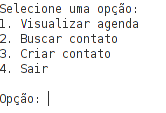
\includegraphics[width=0.5\linewidth]{1}
\end{center}
   \caption{Menu inicial de navegação da agenda telefônica digital.}
\label{fig:long}
\label{fig:onecol}
\end{figure}

De acordo com a Figura 1, as opções são mostradas e o usuário consegue escolher a opção desejada digitando o valor associado a mesma, a partir de sua escolha o usuário é direcionado para a próxima tela.

\subsection{Arquivo Texto}

A Figura 2 representa a maneira como os registros criados estão armazenados no arquivo txt e sua formatação, cada registro encontra-se em uma linha e cada informação do mesmo está separada pelo delimitador ;. Não foi permitido espaços vazios entre as informações, nem que os \textbackslash0 e \textbackslash n fossem escritos no arquivo texto.

\begin{figure}[ht]
\renewcommand{\figurename}{Figura}
\begin{center}
   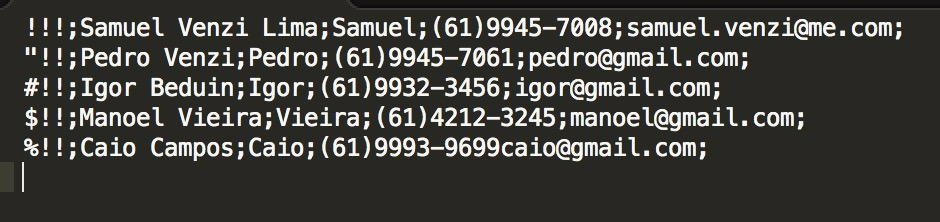
\includegraphics[width=1.0\linewidth]{2}
\end{center}
   \caption{Arquivo de texto "db.txt"}
\label{fig:long}
\label{fig:onecol}
\end{figure}

\subsection{Percentuais de Utilizaçao das Instruções}

A Tabela 7 mostra a proporção em cada função implementada dos tipos de instruções. Tal que, \textit{ALU} são instruções que utilizam a Unidade Lógico Aritmética (add, sub, entre outras), \textit{Jump} são instruções de salto incondicional (j, jal, jr), \textit{Branch} são instruções de salto condicional (beq, bne, blt), \textit{Memory} são instruções de acesso à memória (lw, lb, sw, sb), e \textit{Other} instruções que não se encaixam nas categorias anteriores.
Essas informações foram obtidas com a utilização da ferramenta \textit{Instruction Statistics}. É interessante notar que essas informações podem ser úteis para realizar otimização de código, entretanto devem ser utilizadas somente como noção básica das principais categorias de instruções utilizadas.

\begin{table}[h]
\renewcommand{\tablename}{Tabela}
\begin{center}
\begin{tabular}{|l|c|c|c|c|c|}
\hline
Parâmetro & Buscar & Visualizar & Editar & Deletar & Criar \\
\hline\hline
\textit{ALU} & 39\% & 39\% & 38\% & 37\% & 39\%\\
\textit{Jump} & 13\% & 13\% & 13\% & 14\% & 13\%\\
\textit{Branch} & 28\% & 28\% & 29\% & 28\% & 28\%\\
\textit{Memory} & 15\% & 15\% & 17\% & 17\% & 15\%\\
\textit{Other} & 5\% & 5\% & 4\% & 4\% & 5\%\\
\hline
\end{tabular}
\end{center}
\caption{Organização dos registradores MIPS.}
\end{table}

%------------------------------------------------------------------------
\section{Discussão e Conclusão}

O produto final deste projeto foi uma agenda digital que permite ao usuário criar, editar, procurar e deletar contatos. Os resultados mostram que, de fato, estatisticamente, a maior quantidade de instruções usadas são as instruções que utilizam a Unidade Lógico e Aritmética (ULA). 

Através dos diversos requisitos realizados no desenvolvimento deste projeto, é notória a diferença na abordagem da linguagem de montagem em relação às outras linguagens de alto nível. Percebe-se que o programa desenvolvido em uma linguagem de máquina é mais eficiente, uma vez que roda mais rápido, demanda pouco processamento e exige o mínimo de memória.

A linguagem de máquina se mostra necessária e é importante no desenvolvimento de aplicações que demandam eficiência. Neste trabalho foi possível desenvolver uma aplicação e entender as particularidades de se programar em uma liguagem \textit{assembly}, além disso este aprendizado é essencial no entendimento da construção dos processadores estudados na disciplina de OAC.

\bibliography{bibl}
\bibliographystyle{harvard}
\begin{thebibliography}{xx}
\bibitem{}\textit{Patterson, D.A., Hennessy, J.L.,Computer Organization and Design – The
Hardware/Software Interface, Fourth Edition, Mourgan Kaufmann, 2009;}
\bibitem{}
\textit{Stalling, W. Arquitetura e Organização de Computadores, 5 ed., Pearson
Hall, 2002;}
\bibitem{}
\url{http://www.mrc.uidaho.edu/mrc/people/jff/digital/MIPSir.html}
\end{thebibliography}

\end{document}
